\documentclass{standalone}
% \documentclass{article}

\usepackage{tikz}

\begin{document}

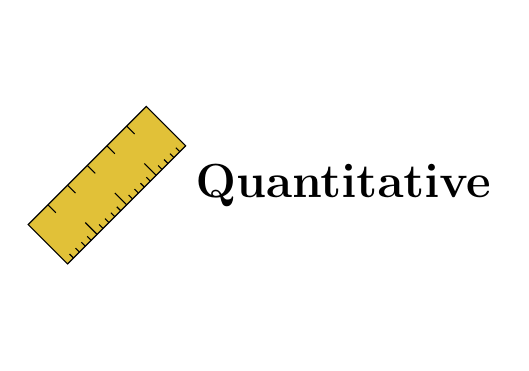
\begin{tikzpicture}
\draw[draw=none, fill=none] (0, -1) rectangle (6, 3);
\node at (4, 1) {\LARGE{\textbf{Quantitative}}};
\draw[draw=black, fill=yellow!50!brown] (0, 0.5) -- (1.5, 2) -- (2, 1.5) -- (0.5, 0) -- cycle;

\foreach \a in {0.25, 0.5, 0.75, 1.0, 1.25}{
\draw (\a, \a+0.5) -- (\a+0.1, \a+0.4);
}

\foreach \a in {0.575, 0.65, 0.725, 0.8, 0.95, 1.025, 1.1, 1.175, 1.325, 1.4, 1.475, 1.55, 1.7, 1.775, 1.85, 1.925}{
\draw (\a, \a-0.5) -- (\a-0.05, \a-0.45);
}

\foreach \a in {0.875, 1.25, 1.625}{
\draw (\a, \a-0.5) -- (\a-0.15, \a-0.35);
}
\end{tikzpicture}

\end{document}

